\DiaryEntry{Newton Root Finding}{2015-06-28}{Maths}

Find zero(s) for $f(x)$. The basic idea is to start at a point $Q = (x_n,y_n)$ on $f(x)$ and calculate the tangent $g(x)$ to the curve at this point. Find the zero of the tangent $g(x)$ (denoted by $x_{n+1}$) and start all over again.

 

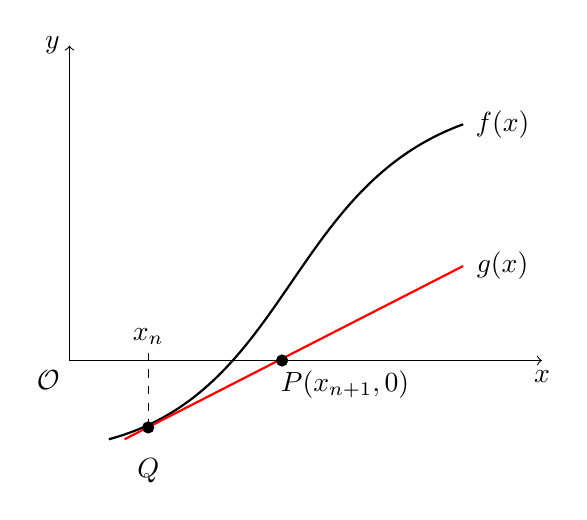
\begin{tikzpicture}

\draw [<->] (0,4) node [left] {$y$} -- (0,0)
node [below left] {$\mathcal{O}$} -- (6.0,0) node [below] {$x$};

\draw [thick] (0.5,-1) to [out=15, in=200] (5,3);


\draw [red, thick] (0.7,-1) to (5,1.2);

\node at (3.5,-0.3) {$P(x_{n+1},0)$};

\draw [fill] (1.0,-0.85) circle [radius=0.07];
\draw [fill] (2.7,0) circle [radius=0.07];
\draw [dashed] (1.0,-0.85) to (1.0,0.1);
\node at (1.0,0.3) {$x_n$};
\node at (1.0,-1.4) {$Q$};

\node at (5.5,3) {$f(x)$};
\node at (5.5,1.2) {$g(x)$};

\end{tikzpicture}

At the point $x_n$, the slope of $f(x)$ is $f'(x_n)$. The tangent $g(x)$ has the following form $y = g(x) = k x + d = f'(x_n)x + d$. We need to find $d$ such that $f(x_n) = g(x_n)$:

\bee
f(x_n) = f'(x_n) x_n + d \rightarrow d = f(x_n) - f'(x_n) x_n
\eee
%
and the tangent becomes

\bee
g(x) = f'(x_n) x + f(x_n) - f'(x_n) x_n
\eee
%
Finding the zero of the tangent yields

\bee
f'(x_n) x + f(x_n) - f'(x_n) x_n = 0 \rightarrow x = \frac{f'(x_n) x_n - f(x_n)}{f'(x_n)} = x_n - \frac{f(x_n)}{f'(x_n)}
\eee
%
This zero is going to be the starting point for the next iteration; i.e. $x_{n+1} = x_n - \frac{f(x_n)}{f'(x_n)}$.

\subsection{Example}

Consider $f(x) = x^2-4$; then $f'(x) = 2x$ and $x_{n+1} = x_n - (x^2-4)/(2x)$. Implementation in Julia is \href{file:///home/cnovak/src/julia/JuliaStuff/newton.jl}{here} and below:

\begin{verbatim}
function newton_solve(z0)
# solve x^2 - 4 = 0
    z = z0
    for n=1:20
        z = z - (z*2-4)/(2*z)
        println(n, " -> ", z)
    end
    return z
end

println(newton_solve(4))
\end{verbatim}
%
Letting $20$ iterations run (starting at $x_0=3.5$) shows that the algorithm quickly converges to $x=2$.

\begin{verbatim}
1 -> 3.5
2 -> 3.0714285714285716
3 -> 2.722591362126246
4 -> 2.457185626921853
5 -> 2.271124947617549
6 -> 2.151745805619235
7 -> 2.0812236253398755
8 -> 2.0421967642419427
9 -> 2.021534326135688
10 -> 2.0108818599087837
11 -> 2.0054703734730377
12 -> 2.0027426475762127
13 -> 2.001373201741756
14 -> 2.000687071968178
15 -> 2.0003436539605324
16 -> 2.0001718564997053
17 -> 2.000085935632882
18 -> 2.000042969662595
19 -> 2.0000214852928857
20 -> 2.000010742761846
2.000010742761846
\end{verbatim}
